\documentclass[tikz,border=3pt]{standalone}
\usepackage[utf8]{inputenc}
\usepackage[T1]{fontenc}
\usepackage{lmodern}
\renewcommand{\familydefault}{\sfdefault}
\usepackage{sansmath}\sansmath
\usepackage{chemfig}
\usepackage{pgfplots}\pgfplotsset{compat=1.18,/pgf/number format/use comma,/pgf/number format/1000 sep={.}}
\usetikzlibrary{arrows.meta,calc,positioning,decorations.pathmorphing,patterns}
% paleta del sitio
\definecolor{nar}{HTML}{E8680C}\definecolor{narc}{HTML}{FFB35C}\definecolor{hielo}{HTML}{FFF3E8}
\definecolor{tinta}{HTML}{1D1D1F}\definecolor{gris}{HTML}{6E6E73}\definecolor{lila}{HTML}{7C5CF0}
\definecolor{azul}{HTML}{2F6FD6}\definecolor{menta}{HTML}{17A673}\definecolor{coral}{HTML}{E8342A}
\begin{document}
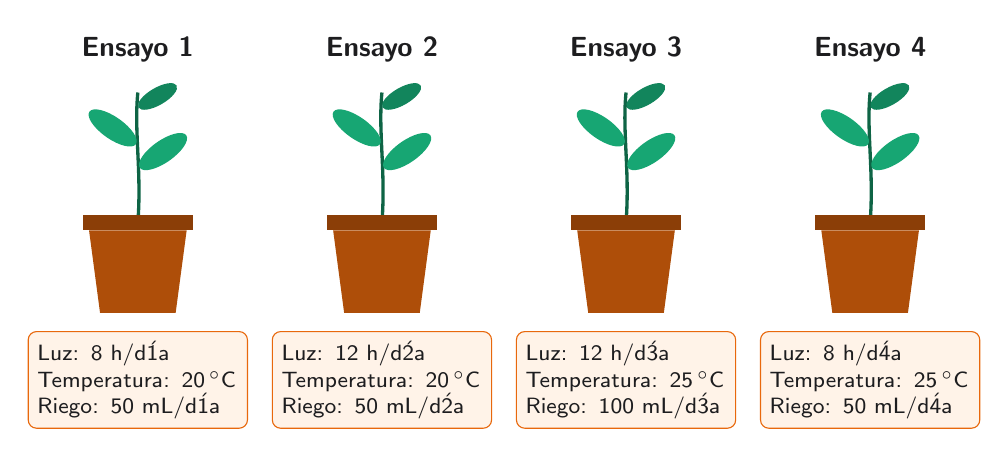
\begin{tikzpicture}[font=\small]
\foreach \i/\luz/\tem/\rie in {1/8/20/50,2/12/20/50,3/12/25/100,4/8/25/50}{
 \begin{scope}[shift={({3.1*(\i-1)},0)}]
  \node[font=\bfseries,text=tinta] at (0,2.35) {Ensayo \i};
  \draw[menta!60!black,very thick] (0,0.15) .. controls (0.05,0.8) and (-0.05,1.3) .. (0,1.8);
  \fill[menta,rotate around={35:(0.32,1.05)}] (0.32,1.05) ellipse (0.36 and 0.14);
  \fill[menta,rotate around={-35:(-0.32,1.35)}] (-0.32,1.35) ellipse (0.36 and 0.14);
  \fill[menta!80!black,rotate around={30:(0.25,1.75)}] (0.25,1.75) ellipse (0.28 and 0.11);
  \fill[nar!75!black] (-0.62,0.05) -- (0.62,0.05) -- (0.48,-1.0) -- (-0.48,-1.0) -- cycle;
  \fill[nar!60!black] (-0.7,0.05) rectangle (0.7,0.25);
  \node[draw=nar,fill=hielo,rounded corners=3pt,align=left,font=\footnotesize,text=tinta,text width=2.55cm] at (0,-1.85)
   {Luz: \luz\ h/día\\Temperatura: \tem\,$^\circ$C\\Riego: \rie\ mL/día};
 \end{scope}}
\end{tikzpicture}
\end{document}
